\documentclass{article}

% if you need to pass options to natbib, use, e.g.:
%     \PassOptionsToPackage{numbers, compress}{natbib}
% before loading neurips_2020

% ready for submission
% \usepackage{neurips_2020}

% to compile a preprint version, e.g., for submission to arXiv, add add the
% [preprint] option:
%     \usepackage[preprint]{neurips_2020}

% to compile a camera-ready version, add the [final] option, e.g.:
%     \usepackage[final]{neurips_2020}

% to avoid loading the natbib package, add option nonatbib:
\usepackage[nonatbib]{neurips_2020}

\usepackage[utf8]{inputenc} % allow utf-8 input
\usepackage[T1]{fontenc}    % use 8-bit T1 fonts
\usepackage{url}            % simple URL typesetting
\usepackage{booktabs}       % professional-quality tables
\usepackage{amsmath}
\usepackage{amsfonts}       % blackboard math symbols
\usepackage{graphicx}
\usepackage{nicefrac}       % compact symbols for 1/2, etc.
\usepackage{microtype}      % microtypography
\usepackage[colorlinks=true, linkcolor=blue, urlcolor=cyan]{hyperref}

\title{Project Report - ECE 176}

% The \author macro works with any number of authors. There are two commands
% used to separate the names and addresses of multiple authors: \And and \AND.
%
% Using \And between authors leaves it to LaTeX to determine where to break the
% lines. Using \AND forces a line break at that point. So, if LaTeX puts 3 of 4
% authors names on the first line, and the last on the second line, try using
% \AND instead of \And before the third author name.

\author{%
  Alexey Grishakov\\
  Electrical and Computer engineering\\
  A17999821\\
  % examples of more authors
}

\begin{document}

\maketitle

\begin{abstract}
This project tests whether a Grassmann-flow language model can serve as an attention-free alternative to a standard causal Transformer at approximately 100M parameters. Instead of token-to-token self-attention, the Grassmann model uses causal geometric mixing with Pl\"ucker coordinates computed from low-dimensional token subspaces. Both models use the GPT-2 tokenizer and the same training setup, so the comparison mainly isolates the effect of the mixing mechanism itself.

At step \(9{,}500\) (about 10 billion tokens, using the same dataloaders for both models), the Grassmann model achieves loss \(5.8413\) and perplexity \(344.23\), compared with Transformer loss \(6.1234\) and perplexity \(456.41\). Total training time was \(12{:}42\) for Grassmann and \(24{:}06\) for the Transformer, making Grassmann roughly \(1.9\times\) faster to train. However, profiling inference with KV caching shows only a modest compute difference between the two, so the main advantage in these experiments is better quality and faster training rather than a clear inference-cost reduction.
\end{abstract}

\section{Introduction}

Most autoregressive language models today rely on self-attention, which scales quadratically with sequence length. As context windows and model sizes increase, this becomes expensive in both memory and compute. The central question of this project is whether attention can be replaced entirely by a geometric flow mechanism while still preserving useful language-modeling quality.

The architecture studied here comes from ``Attention Is Not What You Need'' \cite{chong2025attentionneed}, which proposes replacing attention with Grassmann-flow geometric mixing over token subspaces. Tokens are projected into a lower-dimensional subspace, causal interactions between positions are encoded through Pl\"ucker coordinates, and a learned geometric mixer replaces attention in each block. Rather than only reproducing the mechanism, I evaluate it at a nontrivial scale (\(\sim\!100\)M parameters).

This report compares the Grassmann model against a causal Transformer baseline trained with the same tokenizer and data pipeline. I report held-out loss and perplexity, total training time, inference runtime, and profiled compute scaling.

\section{Related Work}

The main reference for the Grassmann model is the original paper by Chong et al.\ \cite{chong2025attentionneed}, which introduces the idea of replacing self-attention with causal geometric mixing over subspace representations. For the baseline, I use a GPT-style causal Transformer, since it remains the standard architecture for language modeling at this parameter scale. Training data comes from a FineWeb-derived corpus \cite{penedo2024the}, a commonly used large-scale web-text dataset.

Earlier work on language-modeling benchmarks has also shown that prediction quality can depend on long-range discourse context rather than only local n-grams \cite{paperno2016lambadadatasetwordprediction}. I kept this in mind when designing the evaluation: both models share the same tokenizer and data pipeline and are trained on the exact same sequence of tokens, making the comparison as direct as possible.
\section{Method}

\subsection{Model setup}
Both models use the GPT-2 tokenizer (\(50{,}257\) vocabulary items), context length \(1024\), and tied input/output token embeddings. The main Grassmann run has approximately \(102.47\)M parameters, with:
\begin{itemize}
    \item \(d_{\text{model}}=640\), \(n_{\text{layers}}=16\), \(d_{\text{ff}}=2560\),
    \item geometric rank \(r=24\), projection width \(d_{\text{geom}}=256\),
    \item causal offsets \(\{1,2,4,8,16,32,64\}\).
\end{itemize}

The Transformer baseline is size-matched and trained with the same data pipeline and optimizer schedule for a fair comparison.

\subsection{Causal Grassmann block}
For each token position \(t\), the model computes geometric features only from past offsets \(t-\Delta\), preserving autoregressive causality. Given reduced vectors \(z_{t-\Delta}\) and \(z_t\), pairwise antisymmetric products define a Pl\"ucker feature vector:
\[
p_{ij}^{(\Delta)}(t) = z_{t-\Delta,i}z_{t,j} - z_{t-\Delta,j}z_{t,i}, \quad i<j.
\]
These normalized geometric features are projected back to model width, aggregated across offsets, and mixed with the current hidden state through a learned gate, followed by a standard FFN residual path.

\subsection{Why this behaves like attention}
The description of what the ``Grassmann'' LM architecture above explains what the block computes, but it is not clear why this can replace attention. In a standard causal attention layer, the current token forms a query, compares it against previous keys, and then uses those similarity scores to build a weighted combination of previous values. The output is therefore content dependent: the representation at position \(t\) changes depending on which earlier tokens are most compatible with the current token.

The Grassmann block keeps that same high level idea of content-dependent retrieval, but changes the mechanism. Instead of scalar query-key scores, it compares the current reduced vector \(z_t\) with a small set of previous reduced vectors \(z_{t-\Delta}\) through antisymmetric Pl\"ucker coordinates. These coordinates describe the oriented two-dimensional subspace spanned by the pair \((z_{t-\Delta}, z_t)\). Intuitively, the model is not asking ``how similar are these two tokens?'' but rather ``what geometric relation do these two token directions form together?'' A learned projection then maps that relation back into the model space.

This creates attention-like behavior in three steps. First, the geometric feature for offset \(\Delta\) depends on both the current token and the earlier token, so the interaction is still content dependent rather than fixed. Second, different offsets can produce different projected updates, so the model can emphasize different kinds of past context depending on the present token. Third, the gate combines the geometric update with the current hidden state, which plays a role similar to deciding how much retrieved contextual information should influence the next representation.

There is also an important difference from Transformer attention. My implementation does not score \emph{all} previous positions and normalize them with a softmax. It only looks at the fixed causal offsets \(\{1,2,4,8,16,32,64\}\), computes one Pl\"ucker-based interaction for each available offset, and averages the resulting updates. So the Grassmann mixer is attention-like because it performs token-dependent contextual mixing, but it is not full attention: it is a sparse geometric retrieval rule over selected past positions. This is exactly why it can be cheaper and more structured, but it is also why long-range information outside those offsets is missed.

\subsection{Training and evaluation protocol}
Both models are trained with the same tokenization, sequence length, and held-out evaluation windows so that the comparison is controlled. I measure held-out loss and perplexity on the same test windows for both models. I also run context-sensitivity sweeps, total runtime benchmarks, and profiled FLOP counts at different prompt lengths. For compute profiling, both models use KV-cached decode so the numbers reflect actual autoregressive inference.

\section{Experiments}

\subsection{Datasets and data format}
\begin{itemize}
    \item \textbf{Training data:} FineWeb-derived token stream (GPT-2 tokenization, pre-tokenized) \cite{penedo2024the}.
    \item \textbf{Held out evaluation:} Fixed token windows from \texttt{data/test\_tokens.bin} with starts from \texttt{data/test\_starts.npy}.
    \item \textbf{Evaluation approach:} shared sequence length \(1024\), device CUDA, bfloat16 evaluation.
\end{itemize}

\subsection{Benchmarks}
\begin{itemize}
    \item \texttt{eval.py} measures held-out loss/perplexity, a short context sweep, and prompt-generation speed on the same checkpoints.
    \item \texttt{bench.py} measures synthetic-prompt prefill latency and uncached decode throughput across prompt lengths.
    \item \texttt{compute\_profile.py} profiles prefill and KV-cached decode FLOPs as prompt length increases.
\end{itemize}

\subsection{Head to head summary}
Table~\ref{tab:heldout} summarizes the main checkpoint metrics from \texttt{polished\_metrics.csv}. The Grassmann model performs better on held-out loss and perplexity, evaluates faster on the shared held-out set, and reaches its best context-bucket loss at the full \(1024\)-token window.

\begin{table}[ht]
\centering
\small
\caption{Main comparison metrics at step \(9{,}500\), taken directly from \texttt{polished\_metrics.csv}. Grassmann lowers held-out perplexity by about \(24.6\%\), while the Transformer remains much faster in greedy generation throughput.}
\begin{tabular}{lcccccc}
\toprule
Model & Params (M) & Loss & Perplexity & Eval sec & Best ctx & Greedy tok/s \\
\midrule
Grassmann & 102.47 & 5.8413 & 344.23 & 528.09 & 1024 & 73.57 \\
Transformer & 111.60 & 6.1234 & 456.41 & 835.58 & 256 & 197.31 \\
\bottomrule
\end{tabular}
\label{tab:heldout}
\end{table}

\subsection{Training time and runtime comparison}
Training was noticeably faster for the Grassmann model: \(12{:}42\) (hours:minutes) versus \(24{:}06\) for the Transformer. That is about \(1.90\times\) faster, or a \(47.3\%\) reduction in total training time.

Inference shows a different pattern. At short prompts the Transformer is clearly faster, but the gap shrinks as context length grows and reverses at \(1024\) tokens in my benchmark.

Figure~\ref{fig:runtime_scaling} comes from \texttt{bench.py}, which uses synthetic token prompts, batch size \(1\), and \(64\) generated tokens per decode run. The plot shows a mixed result: the Transformer is much faster for short prompts and still leads on uncached decode throughput, but Grassmann's prefill curve grows more slowly and is faster at the longest tested prompt (\(24.96\) ms vs.\ \(36.22\) ms at length \(1024\)).

\begin{figure}[ht]
\centering
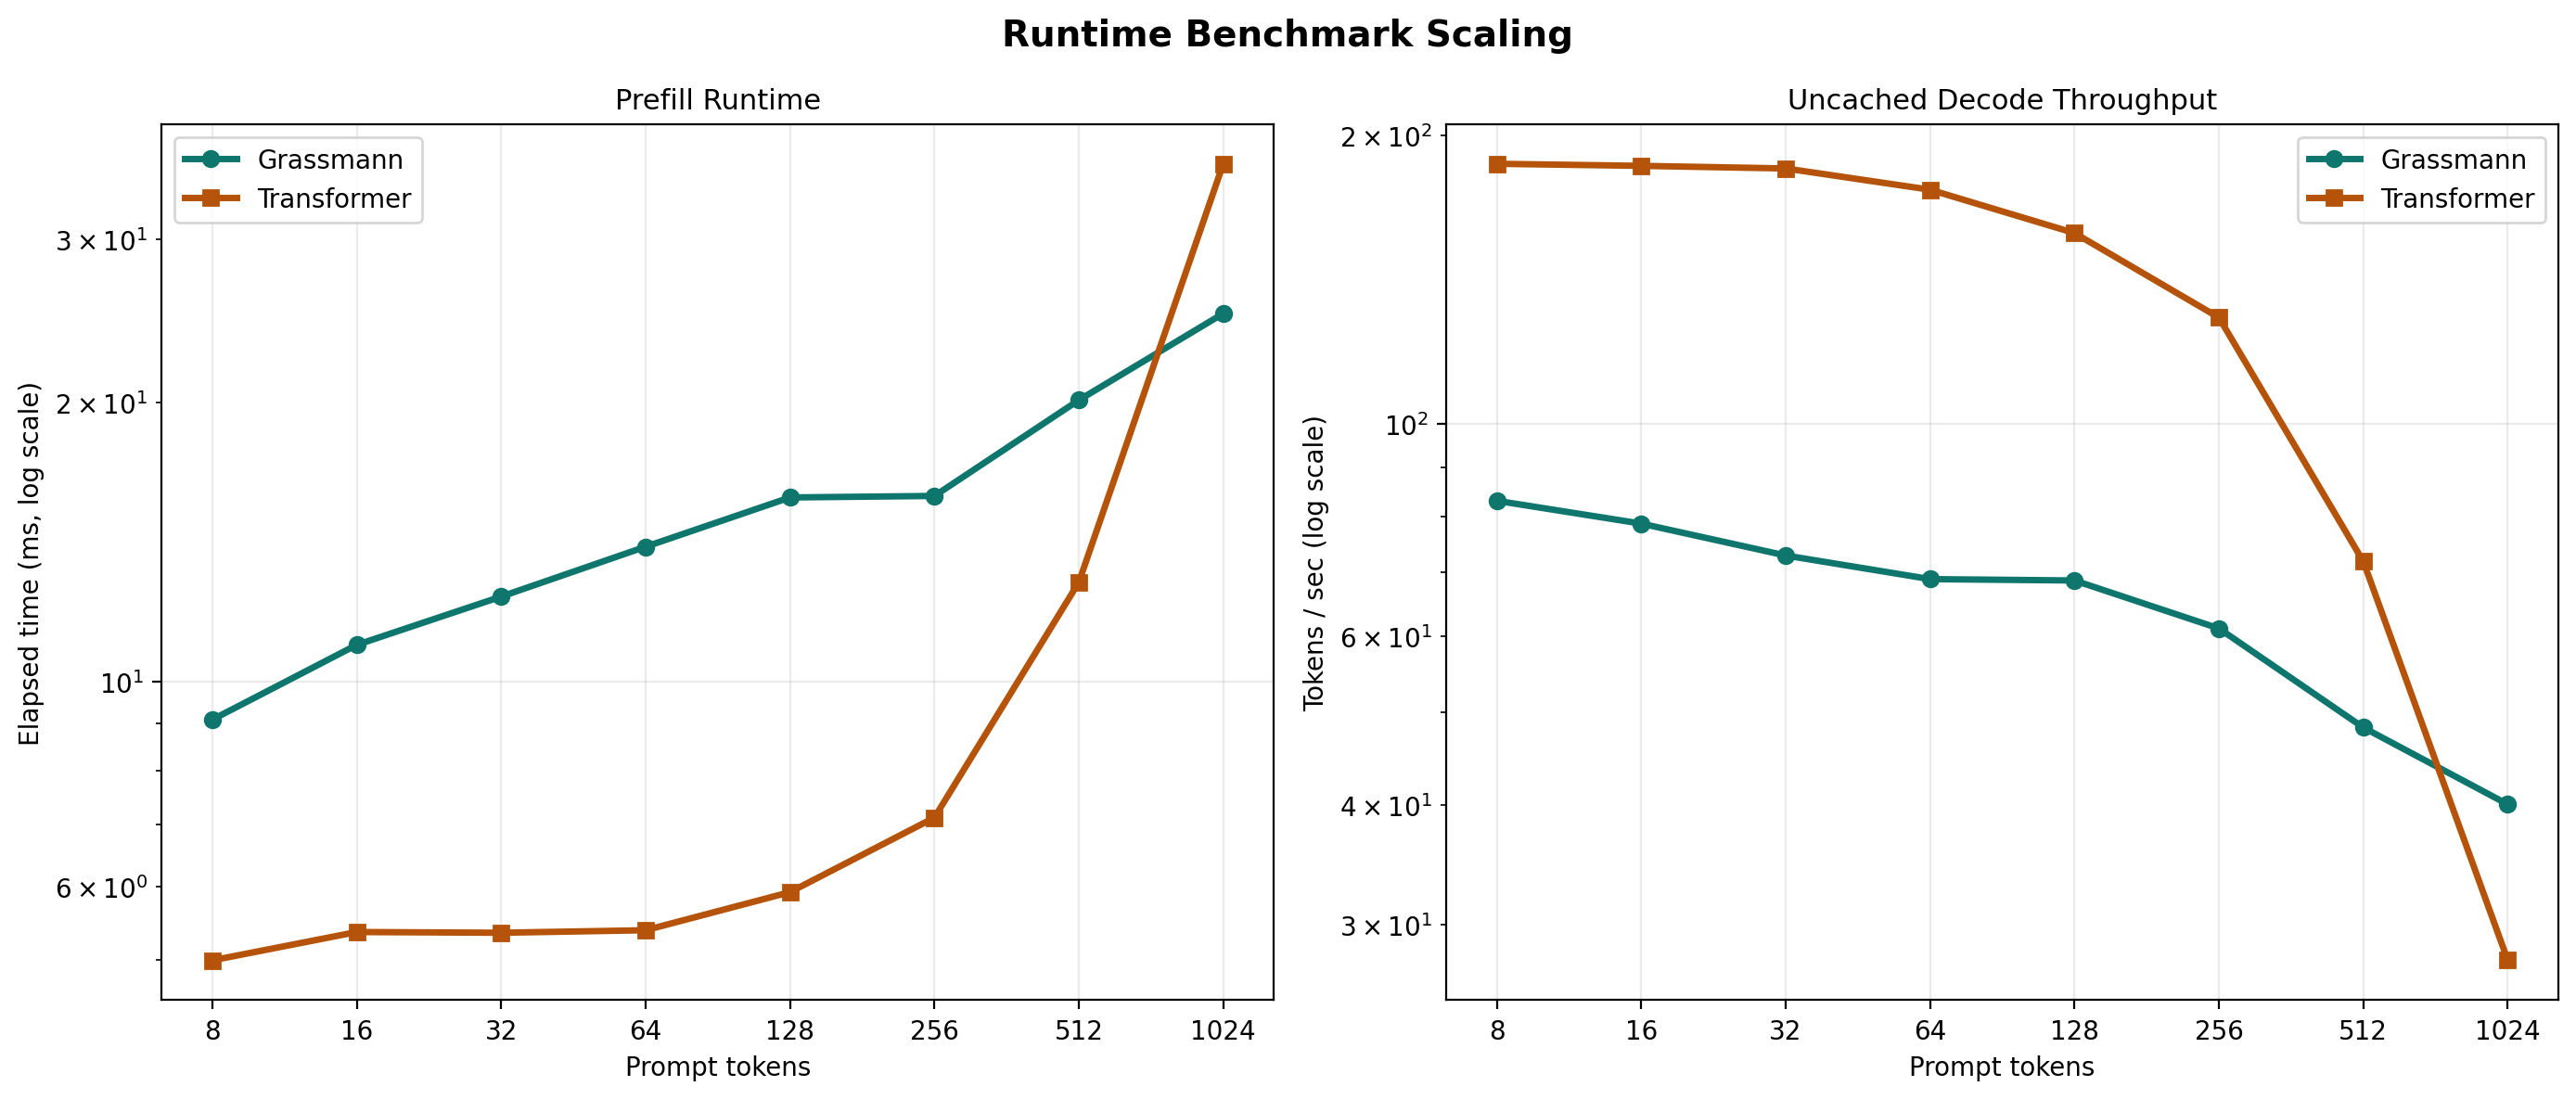
\includegraphics[width=0.92\linewidth]{../code/eval_runs/default_benchmark/runtime_scaling.png}
\caption{Runtime scaling from \texttt{bench.py}. Left: prefill latency versus prompt length. Right: uncached decode throughput for \(64\) generated tokens.}
\label{fig:runtime_scaling}
\end{figure}

There is therefore a clear trade-off. The Transformer is faster at short contexts, likely because attention kernels are currently better optimized. Grassmann catches up as the prompt grows longer and is faster on prefill at \(1024\) tokens. However, the practical speed advantage only appears near the top of the tested range. Further experiments with substantially larger context windows would be needed to determine whether the Grassmann model realizes a more decisive linear-scaling advantage over the Transformer's quadratic prefill cost.

\subsection{Context sensitivity comparison}
Both models were evaluated by scoring a fixed suffix while varying the visible prefix length. Grassmann is more stable across context lengths, while the Transformer shows a larger improvement as context increases before flattening out.

Grassmann has better loss at every tested context length, from \(5.8317\) at \(32\) tokens to \(5.8302\) at \(1024\). At the same time, its numbers barely change as context grows: the spread from \(32\) to \(1024\) is very small. The Transformer, by contrast, improves more noticeably from \(6.1180\) at \(32\) to \(6.0990\) at \(256\) before leveling off and slightly worsening again by \(1024\). This suggests that the Grassmann model may not be using long-range context as effectively as the Transformer, even though its absolute quality is better.

This matters because prior work \cite{paperno2016lambadadatasetwordprediction} has shown that some predictions genuinely depend on long-range discourse context rather than only local patterns. That concern is also consistent with the current implementation: the model uses predefined look-behind offsets, so it cannot directly mix information from arbitrarily far back in the sequence. This is a real limitation at larger context windows, because tokens outside that offset pattern are effectively invisible to the geometric mixer.

\subsection{Profiled compute scaling with KV cache}
To separate raw runtime from operation-level compute cost, I also profiled FLOPs as prompt length increases. Figure~\ref{fig:profiled_compute} comes from \texttt{compute\_profile.py}; its prefill panel runs out to \(1024\) tokens, while the cached decode panel profiles \(16\) generated steps up to prompt length \(256\). The decode study uses the cached autoregressive path for both models, so it reflects inference with KV cache rather than naive recomputation. This matters because, without KV caching, my implementation of the Grassmann-flow model would drift back toward quadratic behavior rather than the intended linear-in-context decode path. The two models track each other closely in both panels: at length \(1024\), prefill is \(254.64\) GFLOPs for Grassmann versus \(270.07\) GFLOPs for the Transformer, while at decode length \(256\) Grassmann is slightly higher (\(66.40\) vs.\ \(62.92\) GFLOPs).

\begin{figure}[ht]
\centering
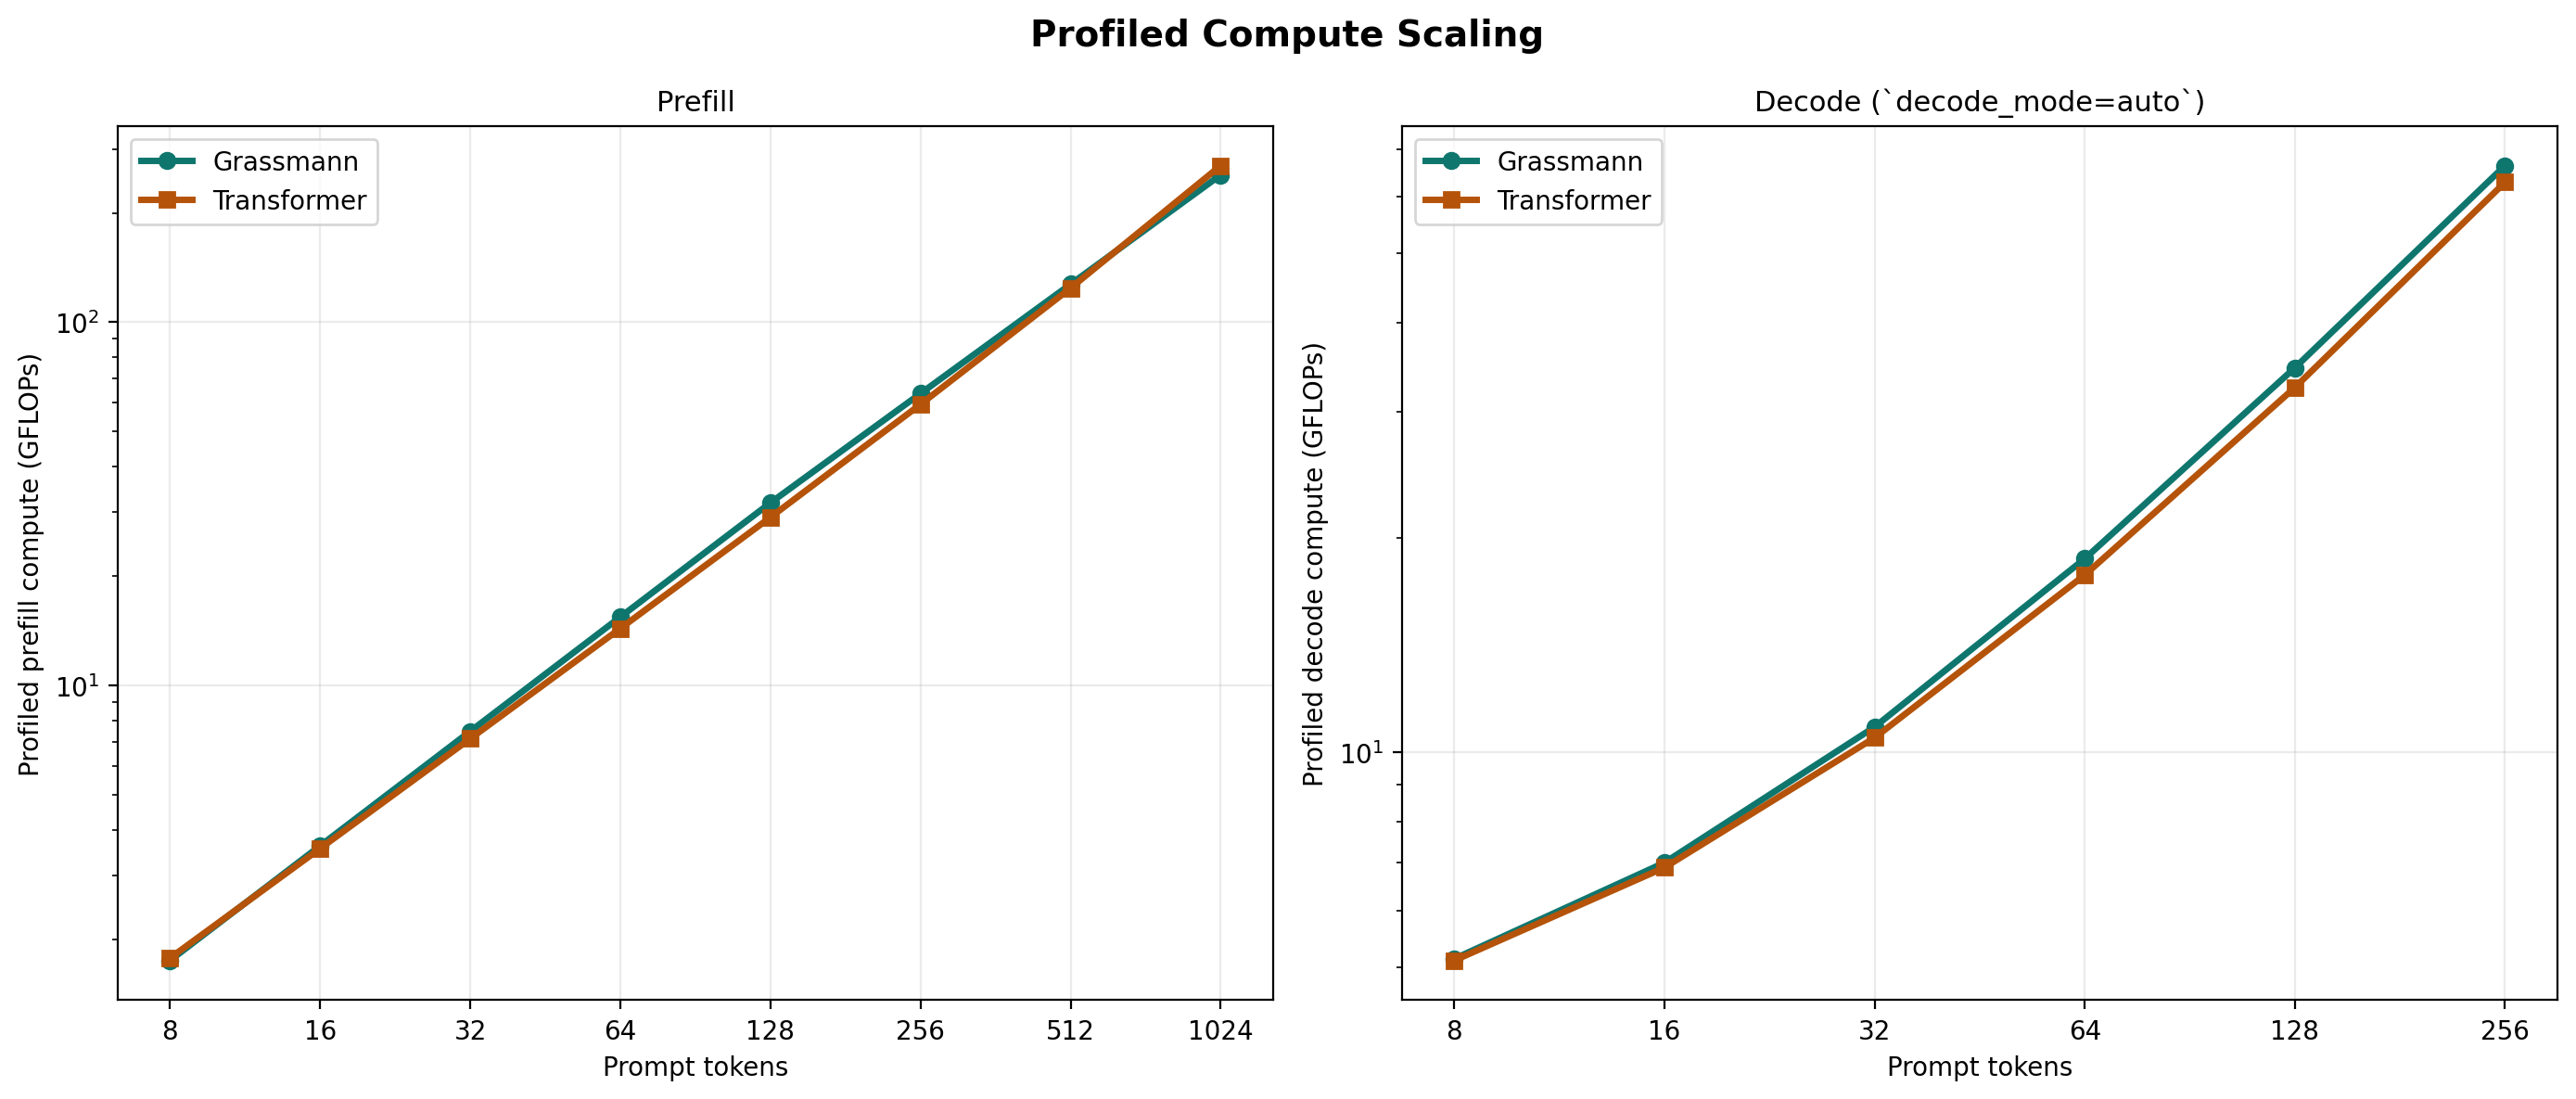
\includegraphics[width=0.92\linewidth]{../code/eval_runs/profiled_compute/profiled_compute.png}
\caption{Profiled compute scaling from \texttt{compute\_profile.py}. Left: prefill FLOPs versus prompt length. Right: KV-cached decode FLOPs for \(16\) generated steps.}
\label{fig:profiled_compute}
\end{figure}

These profiles are worth examining carefully because they tell a somewhat different story from the overall runtime numbers. When both models use KV cache, the FLOP difference between them is quite small. Prefill FLOPs are close, and cached decode FLOPs are also close, with Grassmann even slightly higher at some prompt lengths. In these experiments, the main benefit of Grassmann is therefore not lower inference FLOPs, but better quality and faster training.

\subsection{Discussion}
The final comparison shows that Grassmann flow is a viable attention-free alternative at this scale. Its main benefits in this project are:
\begin{itemize}
    \item better quality on held-out data than the size-matched Transformer baseline; held-out perplexity improves by about \(24.6\%\)
    \item substantially shorter total training time in the current implementation,
    \item competitive long context runtime, with an advantage appearing at the longest tested prompt.
\end{itemize}


That said, there are clear caveats. Once both models use KV cache, the FLOP difference during decode is small, so the Grassmann model does not have a large practical inference-compute advantage. It is also slower than the Transformer at short contexts, and the context-sensitivity results suggest that it may not be taking full advantage of long-range information in this checkpoint.

Overall, geometric mixing can outperform a standard Transformer on quality and training efficiency at 100M parameters, but it is not an obvious win on inference cost. It is difficult to tell how much of that is fundamental to the architecture versus specific to my implementation. Testing with a larger context window would be a natural next step, since \(1024\) tokens is still relatively short and the linear-versus-quadratic scaling difference should become more pronounced on longer sequences.

One possible niche is smaller models that do not require very large effective contexts. In that setting, Grassmann flow may offer better training speed while still improving the quality of early-token predictions. However, the practical use cases remain unclear in the current state of the model. In my benchmarks, the advantages over a classical Transformer appear only in some long-context settings, and the fixed-offset geometric mixer cannot directly incorporate information from the earliest tokens once they fall outside the offset pattern.


\section{Supplementary Material}

Additional materials for the report:
\begin{itemize}
    \item Training, evaluation, and benchmarking code written entirely by me (the original paper did not provide implementation code),
    \item Benchmark logs,
    \item \href{https://replacethiswithvideolink}{Demo video}
    \item \href{https://github.com/grishnakov/176-final-project-alexey-grishakov}{GitHub repository}
\end{itemize}

\bibliographystyle{IEEEtran}
\bibliography{mybib}


\end{document}
